\documentclass[orivec,envcountsame]{llncs}

\usepackage{amsfonts, amssymb}
\usepackage{amsmath}
\usepackage{array}
\usepackage{booktabs, tabularx}
\usepackage[T1]{fontenc}
\usepackage{fullpage}
\usepackage{lmodern}
\usepackage{graphicx}
\usepackage{booktabs}
\usepackage{diagbox}
\usepackage[colorlinks=true,
            citecolor=blue,
            linkcolor=blue,
            urlcolor=blue,
            pdfstartview=FitH,
            bookmarks=true,
            bookmarksopen=true,
            bookmarksdepth=2,
            ]{hyperref}
\usepackage{xspace}
\newcommand{\ra}[1]{\renewcommand{\arraystretch}{#1}}
\usepackage{multirow}
\usepackage{enumerate}
\usepackage{xcolor}
\usepackage{todonotes}
\usepackage{csquotes}
\usepackage{algorithm,algpseudocode}

\title{Snapping mechanism}
\author{Dan Ristea}
\institute{
  University College London, \email{dan.ristea.19@ucl.ac.uk}
}

\begin{document}

\maketitle

\pagebreak
\section{Introduction}
\todo[inline]{write an intro}
\section{Background}
\subsection{Differential privacy}
Differential privacy is a property of a mechanism for aggregate data retrieval which protects individuals' data by making any observed output of a mechanism almost as likely as the output of the mechanism if any one record is not present. Differential privacy was first introduced by Dwork et al. in 2006~\cite{dwork_calibrating_2006}.

$Pure$ differential privacy or $\epsilon$-differential privacy quantifies the privacy loss to an individual with the parameter $\epsilon$, also referred to as the \textit{privacy budget}.

\begin{definition}
A randomised mechanism $M$ is said to have $\epsilon$-differential privacy if for all neighbouring databases $X$ and $Y$, and for all events $S \subseteq$ Range$(M)$, the following inequality holds:

\large $$\Pr[M(X) \in S] \leq e^\epsilon * \Pr[M(Y) \in S] \footnote{$e^\epsilon \approx 1 + \epsilon$ for values of $\epsilon$ close to $0$}$$
\end{definition}

Neighbouring databases $X, Y$ are defined with respect to a distance metric $d$ as having $d(X, Y) = 1$. The distance metric is dependent on the type and structure of the data. In typical database applications where each individual's data is represented as a single row, the distance metric used is the $L_1$ distance. Two datasets are neighbours with respect to $L_1$ distance if they only differ by the inclusion or exclusion of one individual's data~\cite{dwork_calibrating_2006}. The definition of neighbours is symmetrical, therefore, the inequality in the definition of DP must hold if X and Y are swapped.

\subsection{Laplace mechanism}

The Laplace Mechanism is an additive mechanism for differential privacy which perturbs the result of a numerical query by sampling from a Laplace distribution parametrised by the privacy budget and the sensitivity of the query.

\begin{definition}
The sensitivity of a query $f$, with regards to a distance metric $d$ is defined as:
\large $$\Delta(f) = \max_{X,Y}(d(f(X), f(Y)))$$
\normalsize where $X, Y$ are neighbouring databases in the domain of $f$.
\end{definition}

When there is no need to differentiate between the sensitivity of multiple functions and the query function is clear from context, sensitivity can be denoted as just $\Delta$.

\begin{definition}
The Laplace distribution is a continuous distribution characterised by probability density function (PDF):
\large $$f_{Lap}(x) = \frac{1}{2\lambda}e^{-\frac{|x - \mu|}{\lambda}}$$
\normalsize where $\lambda$ is the scale of the distribution and $\mu$ is the mean.
\end{definition}


\begin{definition}
The $\epsilon$-differentially private Laplace Mechanism $M_{Lap}$ applied to a query $f: \mathcal{D} \rightarrow \mathbb{R}$ of sensitivity $\Delta$ on a database $D \in \mathcal{D}$ is given by:
\large $$ M_{Lap}(D, f) = f(D) + X $$
\normalsize where $X$ is sampled from the Laplace distribution with mean 0 and and scale $\lambda = \frac{\Delta}{\epsilon}$.
\end{definition}


In practice, to sample a Laplace random variable with scale $\lambda$, the following procedure is used, derived from the inverse cumulative distribution function of the Laplace distribution:
\begin{eqnarray}
X \leftarrow (2Z - 1) \cdot \lambda log(U) \label{eq:lap}
\end{eqnarray}

where $Z$ is a uniformly sampled bit, and $U$ is uniformly sampled from $[0, 1)$.

\subsection{Floating-point specification}
The discrete and finite nature of computers does not allow the full range of real numbers to be represented. The IEEE 754 double-precision floating-point standard or \textit{double} is a format designed to approximately represent real values as a fixed 64-bit format. It introduces a trade-off between precision and the range of numbers that can be represented. Values closer to 0 are able to be more precisely encoded.

A double is composed of a 1-bit sign, 11-bit exponent, and 52-bit significand or mantissa~\cite{IEEE}. For all values of the exponent, other than 0 and 2047, the minimum and maximum, respectively, double values are decoded as:

$$ (-1)^{sign} \times (1.mantissa) \times 2^{exponent-1023} $$

An exponent of 0 designates a \textit{subnormal} value, which allows for smaller values, closer to 0, to be encoded.

$$ (-1)^{sign} \times (0.mantissa) \times 2^{-1022} $$

This representation allows for a precision of approximately 16 decimal digits, so real values must be approximated to the nearest representable double-precision floating-point number. The maximum relative error introduced by the rounding is called the \textit{machine epsilon} and its value depends on the precision of the representation. A 64-bit double-precision floating-point number, with 53-bit precision (1 bit is implicit) has a machine epsilon of $2^{-53}$.

As done in \cite{mironov2012significance}, we will designate the subset of $\mathbb{R}$ which is representable as a double as $\mathbb{D}$. The representable numbers are not evenly spaced throughout the reals; between any consecutive powers of two in $\mathbb{D}$, only $2^{52}$ evenly-spaced values can be represented. Therefore, the granularity of the values which can be encoded as floating-point numbers differs depending on the exponent. The \textit{unit in the last place (ulp)} is used to denote the numerical value of the least-significant bit in the encoding if it set to a value of 1. In other words, for a given exponent, the \textit{ulp} is the absolute difference in encoded value if the last bit of a floating-point number is changed. Thus, the \textit{ulp} of all floating-point numbers with the same exponent is the same and it can be used to characterise the disjoint sub-sets of $\mathbb{D}$ separated by consecutive powers of 2.

\subsection{Uniform sampling}
The non-uniform distribution of representable values introduces challenges in random sampling. The standard approach to sampling a random number from the interval $\mathbb{D} \cap [0, 1)$ across implementations and languages is to sample a random n-bit integer and divide it by $2^n$. The value of $n$ in C and Python is $53$ (see \textit{Table~1} in~\cite{mironov2012significance} and the \textit{RECIP\_BPF} constant in the Python built-in module \textit{random}), leading to uniform sampling only generating multiples of $2^{-53}$, which are only a small subset of all representable values in $\mathbb{D} \cap [0, 1)$.

\subsection{Floating-point vulnerability}
Although the Laplace mechanism is correct when working with real numbers, 
the particularities described above combine to render it vulnerable~\cite{mironov2012significance}.

If we consider the Laplace sampling technique \ref{eq:lap} as a function from $\mathbb{D} \cap [0, 1)$ to $\mathbb{D}$, fixing the sign and scale, the use of the uniform sampling technique above leads to a small subset of $\mathbb{D} \cap [0, 1)$ being used as input. Therefore, the image of the function after scaling includes only a small subset of the function's domain. This is made worse by rounding, as different input values can be mapped to the same output.

When the Laplace mechanism is applied to a non-zero value, it offsets the image, causing it to not fully overlap with the image of the mechanism applied to 0. As such, if a value is observed as the output of the Laplace mechanism that lies outside the image of the Laplace sampling function \ref{eq:lap}, it constitutes what Mironov terms \textit{"smoking gun evidence"} that the mechanism was applied to a non-zero value. This allow the construction of a distinguisher with a higher probability of discriminating between neighbouring databases than the maximum multiplicative term of $e^\epsilon$ required by differential privacy.

For a more detailed explanation of the underlying mechanism of the attack, see Sections 4.4 and 4.5 of Mironov's paper~\cite{mironov2012significance}.

\subsection{Snapping mechanism}
To differentiate between operations on floating-point numbers from operations on real numbers, Mironov uses the following notation: $\oplus$, $\otimes$, and $\oslash$ to represent floating-point addition, multiplication, and division respectively.

\begin{definition}
The snapping mechanism, parametrised by $\Lambda$ and a bound B, is defined by Mironov~\cite{mironov2012significance} as:
\large $$ M_{snap}(D, f) = clamp_B(\lfloor clamp_B(f(D)) \oplus S \otimes \lambda \otimes LN(U^*)) \rceil_\Lambda) $$
\normalsize where 

$U^*$ is uniformly sampled from $\mathbb{D} \cap [0, 1)$, 

$LN(x)$ is the natural logarithm implemented with exact rounding,

$\lambda = \frac{1}{\epsilon}$,

$\Lambda$ is the smallest power of 2 greater or equal to $\lambda$

$\lfloor x \rceil_\Lambda$ rounds to the nearest multiple of $\Lambda$, with ties broken towards $+\infty$ 

$clamp_B(x) =
\begin{cases}
    B &\quad\text{if x} > B \\
    -B &\quad\text{if x} < -B \\
    x &\quad\text{otherwise} \\ 
\end{cases} 
$
\end{definition}

The above definition assumes the sensitivity of the query is 1. If the sensitivity is not 1, the result of $f(D)$ can be scaled in proportion to the sensitivity. 

Compared to a Laplace mechanism with $\epsilon$-differential privacy, the equivalent snapping mechanism offers $\epsilon + 12B\eta\epsilon + 2\eta$-privacy, where $B$ is the bound and  $\eta$ is the machine epsilon, the maximum relative error introduced by floating-point rounding, which is equivalent to $2^{-53}$ for double-precision floating-point numbers.

The proof that the snapping mechanism is differentially private can be found in Section 5.2 of \cite{mironov2012significance}.


\section{Attack implementation}
The implementation of the attack uses the ideas described in Section 4.5 of the paper~\cite{mironov2012significance}. Although Mironov details the underlying concepts of the attack, the paper does not describe the exact algorithm the attack needs to perform. As such, a description of the steps required to perform the attack is provided below.

The attack can distinguish between values which are the result of applying the Laplace mechanism to 0 and values which are the result of applying the Laplace mechanism to any other value with high probability. In an interactive setting, where the attacker can control the queries, the ability to distinguish between 0 and non-0 values can be used to extract private information from a database which implements the Laplace mechanism for differential privacy to answer queries. An example of an application of this attack is described in Section 4.7 of~\cite{mironov2012significance}, where it is used to reconstruct the text records in a database.

The attack code was written in Python and uses the Numpy numerical library~\cite{harris2020array}, which is written in C. The uniform sampling from $[0, 1)$ in Python and Numpy only produces integer multiples of $2^{-53}$ (see \textit{Table~1} in \cite{mironov2012significance} and the \textit{RECIP\_BPF} constant in the Python built-in module \textit{random}). The attack attempts to determine if an observed output of a Laplace mechanism implementation could have been generated by applying \ref{eq:lap} to an integer multiple of $2^{-53}$ in $[0, 1)$, exploiting the implementation of the uniform distribution in common use. If a value can be found, then it is possible that the observed output was obtained by applying the Laplace mechanism to $0$; otherwise, the mechanism must have been applied to a non-zero value.

The implementation works backwards from the observed output of the differentially private mechanism. It assumes that the observed output is the result of the Laplace mechanism applied to a value of 0 and, therefore, a value sampled from a Laplace distribution wit mean 0. For a given output value $y$ of a Laplace mechanism with scale $\lambda$, the attack starts by finding values $ u \in \mathbb{D} \cap [0, 1)$ such that $|\lambda \otimes log(u)| = |y|$. It does this by inverting the function \ref{eq:lap} used to sample Laplace variables. If the observed value $y$ is positive, its sign is set to negative. As the Laplace distribution is symmetric about its mean, this does not impact the correctness of the algorithm. This simplifies further calculations as the logarithm of sub-unitary numbers is always negative. The value is then normalised by dividing by scale $\lambda$. Finally, a candidate value $u'$ is obtained through exponentiation.

$$u' = exp(-|y| \oslash \lambda)$$

Due to the inaccuracies inherent to floating-point operations, even if the observed value $y$ was the result of applying the Laplace mechanism to $0$, $u'$ may not be a multiple of $2^{53}$. Therefore, to better capture possible value of $u$, the attack checks that the multiples of $2^{53}$ immediately above and below $u'$ can be used to generate $y$. The attack outputs a positive when there exists an integer multiple of $2^{-53}$ in $\mathbb{D} \cap [0, 1)$ such that $|\lambda \otimes log(u)| = |y|$.

Testing the attack using the full range of double-precision floating-point numbers that can be generated by the uniform distribution implementations described above was not feasible within the time available. Therefore, random sampling from the uniform distribution was used to verify the attack. The results of testing 1,000,000 iterations of each implementation with inputs 0 and 1 can be seen in Table \ref{tab:results}.

The attack was tested against a range of implementations: a Laplace mechanism implementation using \textit{np.random.laplace}; the histogram implementation from StatDP, the implementation of a statistical differential privacy violation detector \cite{ding_detecting_2018}; and the Laplace implementation from IBM's Diffprivlib library~\cite{diffprivlib}. When testing the distinguisher's ability to differentiate between $M_{Lap}(0)$ and $M_{Lap}(1)$, it always succeeded in identifying if a value was the result of applying the Laplace mechanism to 0, thus the attack has a recall score of 1. This shows that the distinguisher's probability of success is entirely determined by the probability of a false positive occurring.

\begin{table}[h]
\ra{1.3}
\centering
\caption{Results of running 1,000,000 iterations of the attack against implementations of Laplace mechanism with input 0 and 1 and $\epsilon = .0001$.}
\begin{tabular}{@{}ll@{}ccc@{}ccc@{}cc@{}}
\toprule 
\multicolumn{1}{c}{Laplace implementation} && \multicolumn{2}{c}{Numpy Laplace} && \multicolumn{2}{c}{StatDP histogram} && \multicolumn{2}{c}{IBM Laplace} \\ 
\cmidrule{1-1} \cmidrule{3-4} \cmidrule{6-7} \cmidrule{9-10}
\diagbox[]{Attack input}{Attack prediction}&& $0$ & $1$  && $0$ & $1$  && $0$ & $1$ \\ \hline
$M_{Lap}(0)$ && \multicolumn{1}{r}{1,000,000} & \multicolumn{1}{r}{0} && \multicolumn{1}{r}{1,000,000} & \multicolumn{1}{r}{0} && \multicolumn{1}{r}{1,000,000} & \multicolumn{1}{r}{0} \\
$M_{Lap}(1)$ && \multicolumn{1}{r}{378,608} & \multicolumn{1}{r}{621,392} && \multicolumn{1}{r}{365,893} & \multicolumn{1}{r}{634,107} && \multicolumn{1}{r}{377,496} & \multicolumn{1}{r}{622,504} \\
\bottomrule
\end{tabular}
\label{tab:results}
\end{table}

The relationship between the scale of the Laplace distribution (and thus $\epsilon$) and the probability of the distinguisher succeeding can be seen in Figure \ref{fig:prob}. False positives occur when an observed value of $M_{Lap}(1)$ is also a possible output of $M_{Lap}(0)$. They occur at a rate of $\sim40\%$ for low values of $\epsilon$, decreasing for high values of $\epsilon$. These result corroborate those in Figure 2 of \cite{mironov2012significance}.

\begin{figure}[h]
\begin{center}
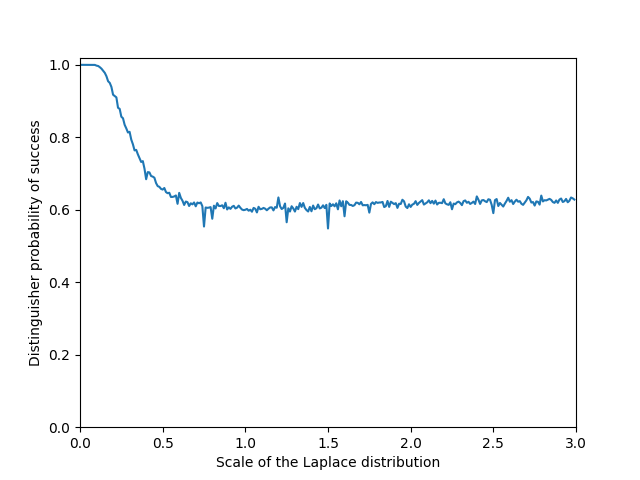
\includegraphics[scale=0.65]{tex/graphics/Probability.png}
\caption{The probability that the attack can distinguish between the Laplace mechanism applied to 0 and the Laplace mechanism applied to 1 as a function of the scale $\lambda=\frac{1}{\epsilon}$ of the Laplace distribution}
\label{fig:prob}
\end{center}
\end{figure}



\section{Snapping mechanism implementation}
As with the attack, the implementation of the snapping mechanism follows the description given by Mironov. As the exact details of the implementation are not provided in \cite{mironov2012significance}, this section describes the steps required to realise the snapping mechanism in Python. The implementation diverges in how bounds are set. Instead of a single symmetric bound, it allows for arbitrary bounds to increase the flexibility of the implementation and potentially reduce the impact the bounds have on the privacy budget.

\subsection{Full-domain uniform sampling and Laplace distribution}
The implementation of uniform distribution in Python's \textit{secrets} and \textit{random} built-in modules, as well as \textit{Numpy}, only produces integer multiples of $2^{-53}$. This is a standard approach across languages and implementations as it requires only 53 bits of randomness compared to the 1074 bits required by full-domain sampling, but distorts a Laplace distribution obtained using the Laplace sampling technique \ref{eq:lap}. The snapping mechanism requires sampling the entire representable space $\mathbb{D} \cap [0, 1)$, which increases the number of possible inputs from $2^{53}$ to $2^{62} - 2^{52}$. 

Initially, the implementation followed the algorithm in Section 5.2 of the paper. The two components of the double are sampled independently. A 52-bit mantissa is randomly sampled as uniform bits. The exponent is sampled using a geometric distribution, making each exponent's probability proportional to its \textit{ulp}, equivalent to the size of the sub-interval of $[0, 1)$ the exponent can encode. The two values were assembled using bit manipulation, then cast to a double-precision floating-point number.

Although this appeared to produce correct results, the Python documentation includes a recently-added example of full-domain uniform distribution~\cite{pythonrandom}, based on a paper by Downey~\cite{downey2007generating}, which present the same methodology as Mironov. As this implementation was peer-reviewed and validated\footnote{See discussion on \url{https://github.com/python/cpython/pull/22664}}, it was adapted for the implementation of the snapping mechanism. Figure \ref{fig:uniform} shows that the implementation of the distribution follows closely the probability density function of the ideal uniform distribution over $[0, 1)$: $f_U(x) = 1$.

\begin{figure}[h]
\begin{center}
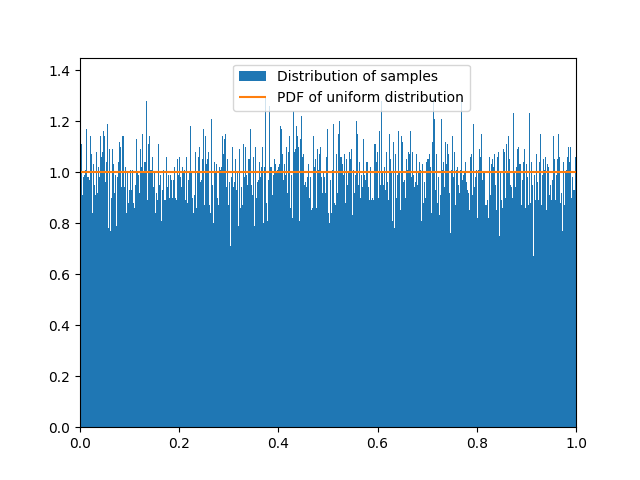
\includegraphics[scale=0.65]{tex/graphics/uniform.png}
\caption{Histogram showing distribution of 1,000,000 samples from uniform distribution implementation compared to the probability density function of the uniform distribution}
\label{fig:uniform}
\end{center}
\end{figure}

Finally, the Laplace distribution is sampled through an implementation of function \ref{eq:lap} using the correctly-rounded natural logarithm function from Crlibm~\cite{lauter_muller_2007,crlibm}, as recommended by Mironov. Figure \ref{fig:laplace} shows that the implementation of the distribution follows closely the probability density function of the ideal Laplace distribution with mean 0.


\begin{figure}[ht]
\begin{center}
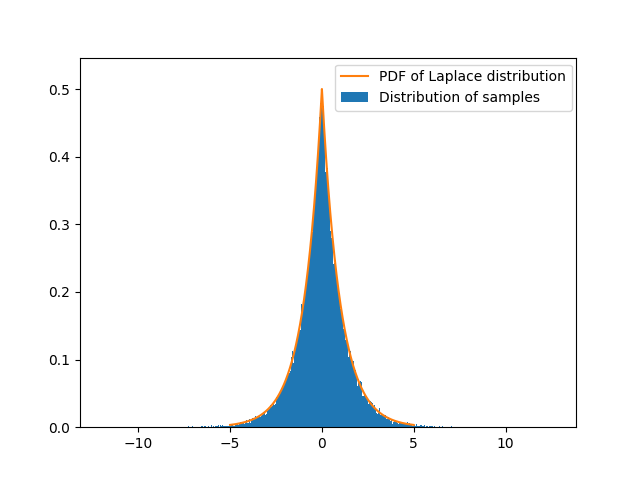
\includegraphics[scale=0.65]{tex/graphics/Laplace.png}
\caption{Histogram showing distribution of 1,000,000 samples from Laplace distribution implementation compared to the probability density function of the Laplace distribution}
\label{fig:laplace}
\end{center}
\end{figure}

\subsection{Scaling input to sensitivity 1 and allowing asymmetric bounds}
The snapping mechanism is defined for query functions that have sensitivity 1. To allow for arbitrary query sensitivity, the query output is scaled inversely proportionally to the sensitivity of the query --$\Delta$-- before the mechanism is applied. The result of the mechanism is scaled back to restore the true sensitivity.

The snapping mechanism is parametrised by bound B, which is symmetrically applied, clamping all outputs to the interval $[-B, B]$. The size of B impacts the privacy guarantee (see Section 5.2 of~\cite{mironov2012significance}) and reduces utility for functions with images that are asymmetric about 0. Therefore, this implementation of the snapping mechanism allows for a lower and an upper bound\footnote{This was inspired by the interface of Diffprivlib's Truncated Laplace implementation \url{https://github.com/IBM/differential-privacy-library/blob/4d48efb6d6086c57d1b813b76b2755c87735d5d8/diffprivlib/mechanisms/laplace.py\#L132}}, which is used to compute a symmetric bound $B$, and to offset the input value before applying the mechanism. The bound must also be scaled by the sensitivity to preserve proportionality. 

$$B := \frac{UpperBound - LowerBound}{2\times\Delta} $$
$$Input' := \frac{Input - LowerBound}{\Delta} - B$$

After the mechanism is applied, the offset is reversed to restore the output of the mechanism to the correct interval.

$$Output := (Output' +B)\times\Delta + LowerBound$$

\subsection{Rounding to nearest power of two}
Finding the value of $\Lambda$, the smallest power of 2 greater than $\lambda$, can be easily performed using bit manipulation of the double-precision floating-point representation of $\lambda$. This is made easier by only working with positive values, where the sign bit is always 0.

For normal floats, checking if a value is a power of 2, can be done by checking if all bits of the mantissa are 0, in which case $\Lambda = \lambda$. Otherwise, the value of $\Lambda$ can be obtained by incrementing by 1 the value of the exponent, and setting the bits of the mantissa to 0. 

Subnormal floats are supported as well, though highly unlikely to occur, as the value of $\epsilon$ would have to exceed $1^{1022}$, which would provide little practical privacy. For subnormal floats, where the exponent is 0, powers of 2 will be encoded as a mantissa with a single bit set to 1, in which case $\Lambda = \lambda$. Otherwise, $\Lambda$ is obtained by setting to 1 the bit immediately above the most significant bit with a value of 1 and all other bits to 0.

Once the value of $\Lambda$ is known, rounding is performed using floating-point division\footnote{Using the \textit{fmod} function \url{https://docs.python.org/3/library/math.html\#math.fmod}} and manipulation of the remainder. Although this appears to be correct, especially as the divisor is a power of 2, floating-point operations may introduce errors due to rounding. If that is the case and what the impact on the correctness of the algorithm is needs to be evaluated.

\subsection{Evaluation}
To demonstrate that it protects against the floating-point attack, the snapping mechanism implementation was evaluated using the attack code. The evaluation was performed using a sample of 1,000,000 values randomly obtained using the full-domain uniform sampling algorithm described above, as testing the entirety of $\mathbb{D} \cap [0, 1)$ was infeasible. Comparing the results in Table \ref{tab:snapres} with those in Table \ref{tab:results} shows the effects of the snapping mechanism in preventing the attack.

\begin{table}[h]
\ra{1.3}
\centering
\caption{Results of running 1,000,000 iterations of the attack against the snapping mechanism implementation with input 0 and 1.}
\begin{tabular}{@{}ll@{}cc@{}}
\toprule 
\diagbox[]{Attack input}{Attack prediction}&& $0$ & $1$ \\ \hline
$M_{Snap}(0)$ && \multicolumn{1}{r}{221,532} & \multicolumn{1}{r}{778,468} \\
$M_{Snap}(1)$ && \multicolumn{1}{r}{221,525} & \multicolumn{1}{r}{778,475} \\
\bottomrule
\end{tabular}\label{tab:snapres}
\end{table}

Figure \ref{fig:laplacevssnapping} offers an illustrative comparison of the distribution of outputs of the Laplace mechanism with those of the snapping mechanism. The visualisation shows the effects of the snapping mechanism as implemented: clamping of the output as can be see by the density of snapping mechanism outputs at 0, rounding to multiples of 2, and offsetting the output to be within asymmetric bounds.

\begin{figure}[H]
\begin{center}
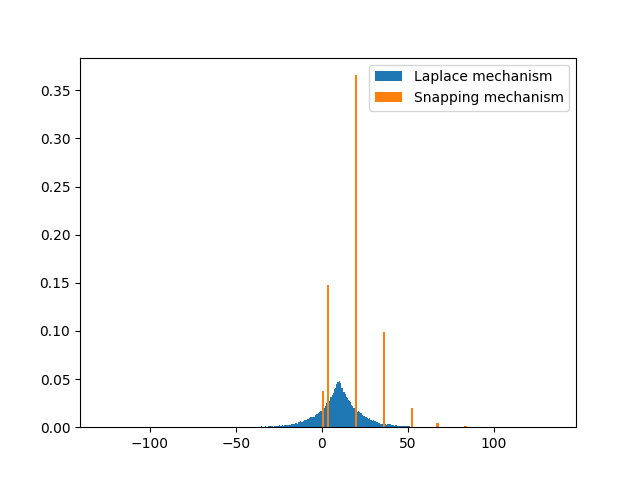
\includegraphics[scale=0.65]{tex/graphics/LaplacevsSnapping.png}
\caption{Histogram showing output distribution of 1,000,000 applications of the Laplace mechanism and of the snapping mechanism to the result of a counting function (sensitivity $\Delta=1$) which outputs 10, with $\epsilon = 0.1$ and snapping mechanism bounds $0$ and $100$ }
\label{fig:laplacevssnapping}
\end{center}
\end{figure}

\subsection{Computing the effective privacy budget}

The privacy guarantee of the snapping mechanism depends not only on the user-set privacy budget $\epsilon$ but also on the size of the bound and the machine epsilon. The snapping mechanism as defined by Mironov provides $\frac{1}{\lambda} + \frac{12 B \eta}{\lambda} + 2 \eta$-differential privacy, where $\eta$ is the machine epsilon, $B$ is the symmetric bound, and scale $\lambda = \frac{\Delta}{\epsilon}$~\cite{mironov2012significance}. 

The above was adapted to this implementation, which allows for arbitrary asymmetrical bound, by computing the equivalent value of the bound and applying the formula above.

$$\epsilon' := \frac{1}{\lambda} + \frac{6\times(UpperBound - LowerBound)\times\eta}{\Delta\lambda} + 2\eta$$

This enables implementations that use a privacy budget accountant to enforce cumulative limits over multiple queries, as is used in \textit{diffprivlib}, to correctly quantify the expended privacy budget of an invocation of the snapping mechanism. It could also allow for a user-set effective privacy budget from which the value of the scale $\lambda = \frac{\Delta}{\epsilon}$ can be derived.

\section{Future work}
The Laplace mechanism implementation found in the \textit{diffprivlib} library~\cite{diffprivlib} provided by IBM is proven to be vulnerable, as demonstrated by the results in Table \ref{tab:results}. The authors of the library are aware of this vulnerability but have not resolved it\footnote{See Github issue: \url{https://github.com/IBM/differential-privacy-library/issues/19}}. I have started adapting the implementation of the snapping mechanism to be used within \textit{diffprivlib}\footnote{See Github draft pull request: \url{https://github.com/IBM/differential-privacy-library/pull/46}} and this is a currently ongoing task.

As the distribution of the Laplace mechanism is symmetrical about the value of the query, the bias of the mechanism is 0. The clamping function used by the snapping mechanism introduces the potential for bias. The bias that can be introduced by the mechanism as designed by Mironov, with symmetric bounds, is dependant on the range of the query function, the scale of the mechanism, and the bound, which is said to be \textit{"exceedingly small"} in some cases, but no precise formula is provided~\cite{mironov2012significance}. The mechanism as implemented here, allows for arbitrary asymmetrical bounds, which, if set correctly, can increase utility, but also allows for user-set bounds that can arbitrarily bias the result. Quantifying the bias of the mechanism depending on the lower and upper bound values and the range of the query function may provide a better understanding of the optimal values of the bounds. As rounding is always performed towards $+\infty$, this may be an additional source of bias to also account for.

As previously mentioned, the rounding step in the mechanism is performed using floating point division. As the divisor is a power of two, the division may not introduce any errors as implemented but it requires additional work to prove or to find a technique that does not introduce any error.

\newpage
\bibliographystyle{splncs03}
\bibliography{references}

\end{document}
